% DOC SETTINGS ===================================
\documentclass{article}
\usepackage[utf8]{inputenc}
\usepackage{fancyhdr}
\pagestyle{fancy}
\usepackage{geometry}
 \geometry{
 a4paper,
 total={170mm,257mm},
 left=20mm,
 top=25mm,
 }
\fancyheadoffset{0mm}
\lhead{ECE2564 HW1}
\rhead{Kavin Thirukonda 2021}
\usepackage{steinmetz}
\usepackage{listings}
\usepackage{circuitikz}
\usepackage{mathtools}  
\mathtoolsset{showonlyrefs} 
\cfoot{}
% DOC SETTINGS ===================================
\begin{document}
\section*{Honor Code:}
\begin{center}
    “I have neither given nor received unauthorized assistance on this assignment.”
    
    
\includegraphics[width = .1\textwidth]{Signature.jpg}
\end{center}
\section*{Problem 1 (10 points)}
Convert  these  decimal  numbers  into  8-bit  unsigned  binary  numbers  and  into  2-digit hexadecimal numbers. Show your work to a reasonable extent. Use leading zeroes as needed to pad the precision of your answers. 
\subsubsection*{a. 39}
\begin{align}
    39_{10} &= 00100111_2\\
    &= 27_{16}
\end{align}
\subsubsection*{b. 90}
\begin{align}
    90_{10} &= 01011010_2\\
    &= 5A_{16}
\end{align}
\subsubsection*{c. 175}
\begin{align}
    175_{10} &= 10101111_2\\
    &= AF_{16}
\end{align}
\subsubsection*{d. 183}
\begin{align}
    183_{10} &= 10110111_2\\
    &= B7_{16}
\end{align}
\subsubsection*{e. 240}
\begin{align}
    240_{10} &= 11110000_2\\
    &= F0_{16}
\end{align}
\newpage
\section*{Problem 2 (6 points)}
Convert these 8-bit signed 2’s complement numbers into decimal numbers. 
\subsubsection*{a. 00101101}
\begin{equation}
    00101101_2 = 45_{10}
\end{equation}
\subsubsection*{b. 11010010}
\begin{align}
    11010010_2 &\Rightarrow 00101110_2\\
    &= -46_{10}
\end{align}
\subsubsection*{c. 01011011}
\begin{equation}
    01011011_2 = 91_{10}
\end{equation}
\subsubsection*{d. 11111111}
\begin{align}
    11111111_2 &\Rightarrow 00000001_2\\
    &= -1_{10}
\end{align}
\subsubsection*{e. 10011110}
\begin{align}
    10011110_2 &\Rightarrow 01100010_2\\
    &= 98_{10}
\end{align}
\subsubsection*{f. 00011101}
\begin{equation}
    00011101_2 = 29_{10}
\end{equation}
\newpage
\section*{Problem 3 (7 points)}
Convert these decimal numbers into 8-bit signed 2’s complement numbers. Use leading zeroes as needed to pad the precision of your answers. If you cannot represent a number in the 2’s complement representation using 8 bits, briefly explain why.
\subsubsection*{a. +27}
\begin{equation}
    27_{10} = 00011011_2
\end{equation}
\subsubsection*{b. +43}
\begin{equation}
    43_{10} = 00101011_2
\end{equation}
\subsubsection*{c. +92}
\begin{equation}
    92_{10} = 01011100_2
\end{equation}
\subsubsection*{d. +128}
\begin{center}
    Cannot be represented because there are only eight bits which are not sufficient to represent 128 in the two's complement system.
\end{center}
\subsubsection*{e. -47}
\begin{align}
    -47_{10} &\Rightarrow 00101111_2\\
    &=11010001_2
\end{align}
\subsubsection*{f. -80}
\begin{align}
    -80_{10} &\Rightarrow 01010000_2\\
    &=10110000_2
\end{align}
\subsubsection*{g. -135}
\begin{center}
    Cannot be represented because there are only eight bits which are not sufficient to represent -135 in the two's complement system.
\end{center}
\newpage
\section*{Problem 4 (7 points)}
This semester, we will see many of the devices that you studied in  ECE 2544 play important roles in the context of a microcontroller and its peripherals. It will be important for you to distinguish devices from one another; one effective way to do this is to have a good grasp on their input-output functions. For each device listed below, match it to the definition of its input-output behavior.
\subsection*{Shift Register:} This synchronous sequential device consists of n commonly-clocked and commonly-controlled flip-flops. On a clock trigger, it moves the bits that make up its state in one direction or the other.
\subsection*{Register:} This synchronous sequential device consists of n commonly-clocked and commonly-controlled flip-flops. It is used to hold an n-bit state for one or more clock cycles.
\subsection*{Decoder:} This combinational device has n inputs and $2^n$ outputs. When the circuit receives an n-bit input, exactly one of the $2^n$ outputs is asserted.
\subsection*{Multiplexer:} This combinational device has $2^n$ inputs, n select lines, and one output. When the circuit receives an  n-bit  value  on  its  select  lines,  the  output  takes  on  the  value  carried  by  the input that corresponds to the select value.
\subsection*{Encoder:} This combinational device has $2^n$ inputs and n outputs. When exactly one of the inputs is asserted, the outputs take on a corresponding n-bit value.
\subsection*{Priority Encoder:} This combinational device has $2^n$ inputs and n outputs. When exactly one of the inputs is asserted, the outputs take on a corresponding n-bit value. When more than one of the inputs is asserted, the output takes on an n-bit value that corresponds to whichever one of the asserted inputs has precedence over the other asserted inputs.
\subsection*{Counter:} This synchronous sequential device consists of n commonly-clocked  and  commonly-controlled flip-flops. On successive clock cycles, it moves through a predetermined order of n-bit states. The most common kind of this device moves in an increasing or decreasing order through states that could be interpreted as numeric values.
\newpage
\section*{Problem 5 (8 points)}
\subsection*{a. The definitions in Problem 4 refer to devices as being combinational and sequential. In  the  context  of  digital  logic,  what  is  the  difference  between  a  device  that  is combinational and one that it is sequential?}
\begin{center}
    sequential devices are usually used for storing data and such while combinational are mostly used for performing computations such as addition, subtraction, division, multiplication and others.
\end{center}
\subsection*{b.  What specific element of a sequential device makes it synchronous?}
\begin{center}
    A the distinction between the two have everything to do with the clock. A sequential device is always active and always performing its designated action, which a synchronous device will only operate properly when given the correct conditions and is given a clock cycle to activate it.
\end{center}
\subsection*{c.   Many of the definitions in Problem 4 refer to input and output signals being asserted. In  the  context  of  digital  logic,  what  does  it  mean  for  an  input  or  an  output  to  be asserted?}
\begin{center}
    Assertion is when a output signal is being held at logic-high or logic-low by a CMOS transistors
\end{center}
\subsection*{d.  Explain the  difference between a  signal that  is asserted active-high  and  one  that is asserted active-low.}
\begin{center}
    If a signal is being asserted high then it is held at saturation by logic that is carried out by CMOS transistors which active low is when it is held at ground by that same logic.
\end{center}
\newpage
\section*{Problem 6 (10 points)}
Analyze the circuit containing D flip-flops shown below by giving the value for Q1 and Q2 that  result  from  each  clock  trigger.  The  flip-flops  are  positive-edge  triggered  so  the question  will  ask  about  the  values  at  the  negative  edges,  by  which  time  the  flip-flop outputs should have settled.

At time t = 0, Q1 = 0 and Q2 equal 1. Note that the flip-flops are commonly-clocked.
\begin{center}
    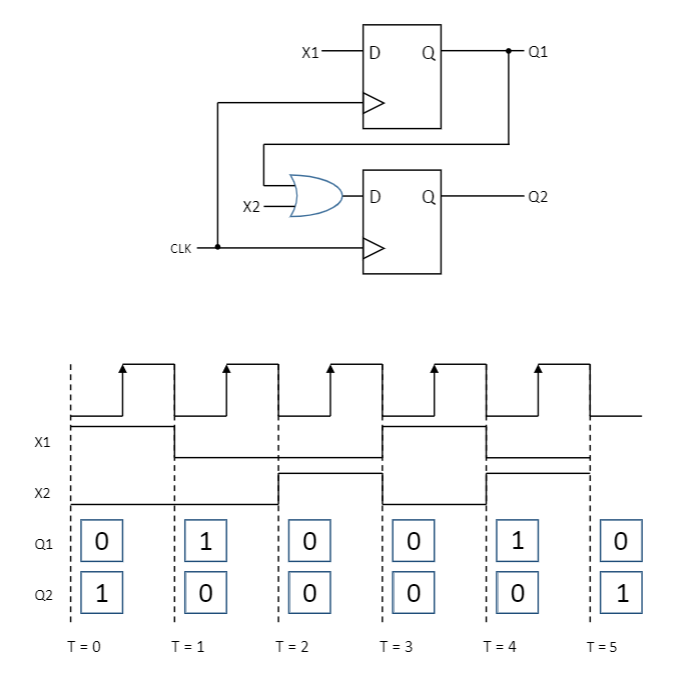
\includegraphics[width = .7\textwidth]{logic.png}  
\end{center}
\newpage
\section*{Problem 7 (12 points)}
The  web  site http://rextester.com  provides  a  convenient  place  to  practice  writing  small programs. To get familiar with it, go to the site and click Run Code, and then select C(gcc) in the drop-down menu under Language. At your first visit, you should see a short program similar to the following:
\lstset{language=C}
\lstset{frame=lines}
\lstset{label={lst:code_direct}}
\lstset{basicstyle=\footnotesize}
\begin{lstlisting}
        //gcc 5.4.0
        #include  <stdio.h>
        main(void){    
            printf("Hello, world!\n");    
            return 0;
        }
\end{lstlisting}
Verify that you can run the program by clicking Run It (F8), near the bottom of the page. After you have become familiar with the interface, write a short program in the C language that creates an array containing the integers 1 through 10, in order. Your program should then compute the sum of the array’s elements. As output, print the array contents and the sum on the screen.  The following is an example of correct program operation.
\begin{lstlisting}
        Contents of array:
        1
        2
        3
        4
        5
        6
        7
        8
        9
        1
        0
        The sum is 55.
\end{lstlisting}
\begin{center}
Pasted code:
\end{center}
\begin{lstlisting}
    //gcc 7.4.0
    
    #include  <stdio.h>
    int main(void){
        int arr[10],sum = 0;
        printf("Contents of array:\n");
        for(int i = 1; i <= 10; i++){ 
            arr[i] = i;
            printf("%d\n", i);
            sum += i;
        }
        printf("The sum is %d.",sum);
        return 0;
    }
\end{lstlisting}
\newpage
\section*{Problem 8 (20 points)}
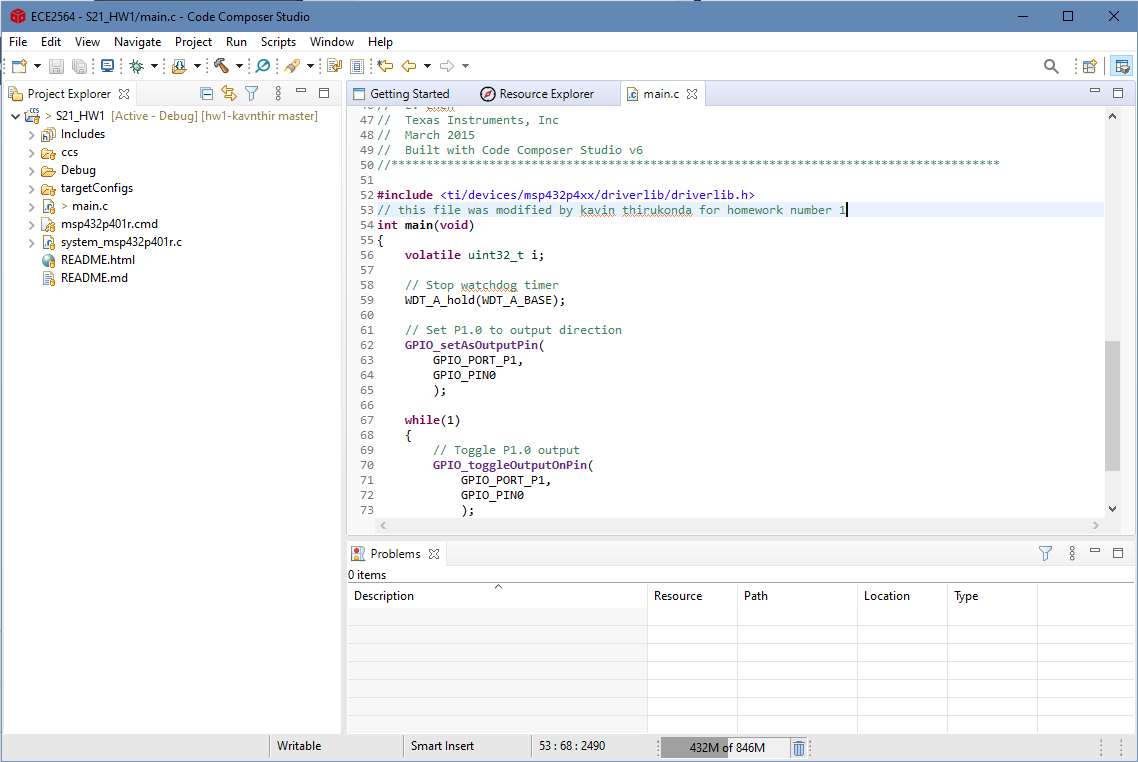
\includegraphics[width = \textwidth]{ccs.png}
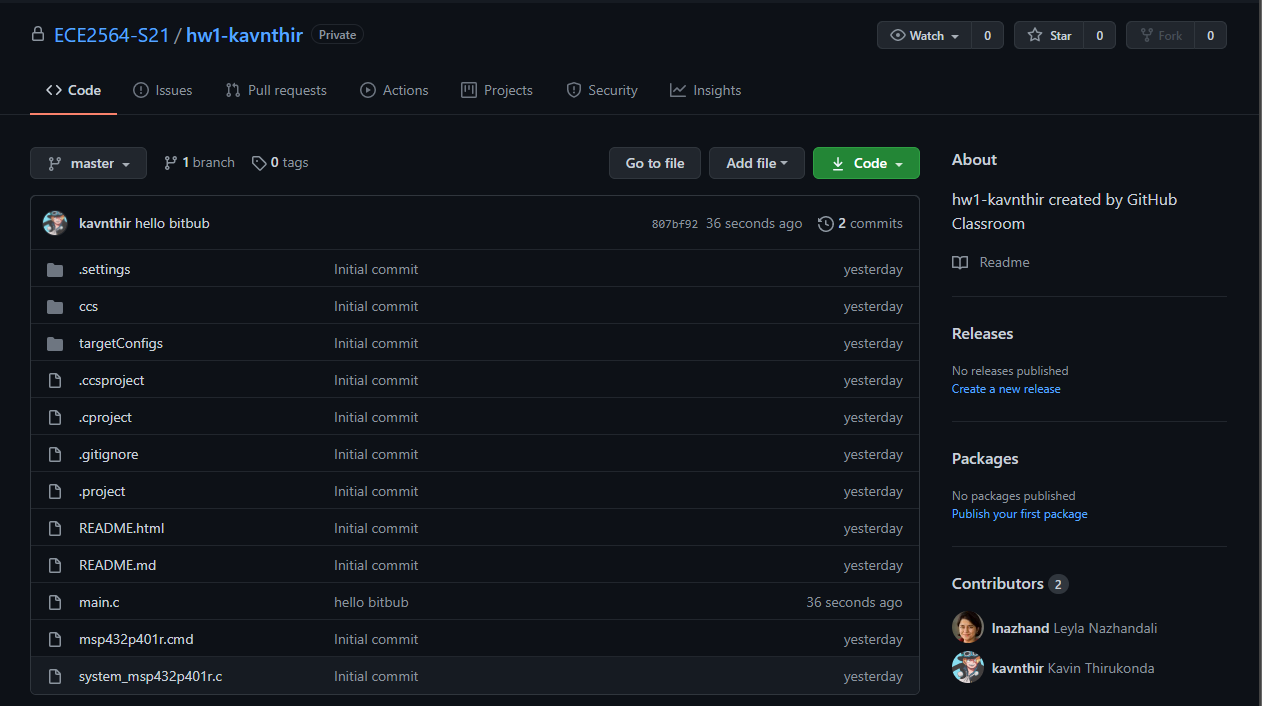
\includegraphics[width = \textwidth]{github.png}
\end{document}
